% ex: ts=2 sw=2 sts=2 et filetype=tex
% SPDX-License-Identifier: CC-BY-SA-4.0

\question Usa la siguiente cuadricula para resolver los siguientes incisos:

  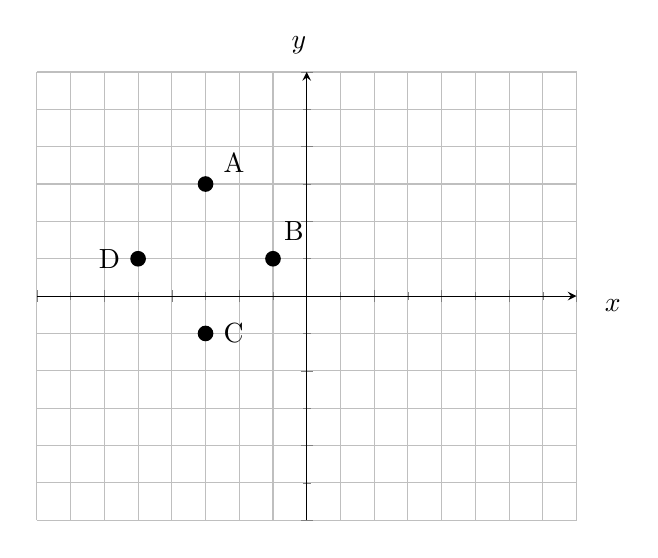
\begin{tikzpicture}
    \begin{axis}[grid=both,ymin=-6,ymax=6,xmax=8,xmin=-8,xticklabel=\empty,yticklabel=\empty,
               minor tick num=1,axis lines = middle,xlabel=$x$,ylabel=$y$,
               label style = {at={(ticklabel cs:1.1)}}]
      \node[label={10:{A}},circle,fill,inner sep=2pt] at (axis cs:-3,3) {};
      \node[label={80:{B}},circle,fill,inner sep=2pt] at (axis cs:-1,1) {};
      \node[label={0:{C}},circle,fill,inner sep=2pt] at (axis cs:-3,-1) {};
      \node[label={180:{D}},circle,fill,inner sep=2pt] at (axis cs:-5,1) {};
    \end{axis}
  \end{tikzpicture}

  \begin{parts}
    \part Encuentra las coordenadas de los vértices en el polígono. \\
    A(\fillin[-3] ,\fillin[3] ) \enspace B(\fillin[-1] ,\fillin[1] ) \\
    C(\fillin[-3] ,\fillin[-1] ) \enspace D(\fillin[-5] ,\fillin[1] ) \\
    \part Traslada la figura 5 unidades a la derecha y 5 unidades hacia
    abajo. (usa la misma cuadricula)
    \part Escribe los nuevos vértices del polígono. \\
    A(\fillin[2] ,\fillin[-2] ) \enspace B(\fillin[4] ,\fillin[-4] ) \\
    C(\fillin[2] ,\fillin[-6] ) \enspace D(\fillin[0] ,\fillin[-4] ) \\
  \end{parts}
